\documentclass{report}
\usepackage[margin=1in, paperwidth=8.5in, paperheight=11in]{geometry}
%Math packages%
\usepackage{amsmath}
\usepackage{amssymb}
\usepackage{amsthm}
%Spacing%
\usepackage{setspace}
\onehalfspacing
%Lecture number%
\newcommand{\lectureNum}{12}
%Variables - Date and Course%
\newcommand{\curDate}{January 30, 2017}
\newcommand{\course}{MATH 239}
\newcommand{\instructor}{Luke Postle}
%Defining the example tag%
%\theoremstyle{definition}%
\newtheorem{ex}{Example}[section]
%Setting counter given the lecture number%
\setcounter{chapter}{\lectureNum{}}
%Package for drawing graphs%
\usepackage{tikz}
\usepackage{verbatim}
\usetikzlibrary{arrows}

\begin{document}
%Note title%
\begin{center}
\begin{Large}
\textsc{\course{} | Lecture \lectureNum{}}
\end{Large}
\end{center} 
\noindent \textit{Bartosz Antczak} \hfill
\textit{Instructor: \instructor{}} \hfill
\textit{\curDate{}}
\rule{\textwidth}{0.4pt}

% Actual Notes%
\subsubsection{Review of Last Lecture}
We defined a \textbf{weighted graph}, which is a graph with a weight function on its edges. From this, we discussed an \textbf{MST} (Minimum Spanning Tree), which is a spanning tree of a weighted graph which has minimum weight over all spanning trees (where weight of $T = \displaystyle \sum_{e \in E(T)} w(e)$. Finally, we mentioned \textbf{Prim's Algorithm} and proved the theorem that:
\begin{center}
\textit{The output of Prim's algorithm in an MST}
\end{center}
Prof. Postle outlined two parts in the proof that may have been confusing and proved them as lemmas:
\subsubsection{Lemma 1}
\begin{center}
\textit{If T is a spanning tree and $e \not\in E(T)$, then $\forall f$ in the unique cycle of $T+e$, $T^\prime = T + e - f$ is a spanning tree}
\end{center}
\textbf{Proof:} $T+e$ is connected because $T$ is. Now, $T^\prime = T + e - f$ is connected because $f$ is in a cycle of $T+e$ and so it's not a bridge. So $T^\prime$ has the same number of components as $T+e$, that is, one.\\
So $T^\prime$ is connected, and $T^\prime$ has no cycles since we deleted the edge $f$, which was in the only cycle. So $T^\prime$ is a tree and is clearly spanning.
\subsubsection{Lemma 2}
\begin{center}
\textit{Let $C$ be a cycle of $G$ and $X$ is a proper, non-empty subset of $V(G)$. Then $\vert E(C) \cap \delta(X) \vert$ is even}
\end{center}
\textbf{Proof (sketch):} Direct $C$ and pair the edges as they go in/out of $X$.

\section{Planar Graphs}
The prettiest topic of Graph Theory, according to Prof. Postle.\\
A graph is \textbf{planar} if it can be drawn in the plane $\mathbb{R}^2$ such that edges go between their ends and edgs do not otherwise intersect (i.e., do not ``cross"). We call such a drawing a \underline{planar embedding} of $G$:
\begin{ex}
A non-planar embedding of a graph (left) and its planar embedding (right)
\end{ex}
%Planar and non-planar graphs%
\begin{center}
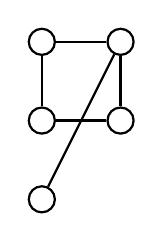
\begin{tikzpicture}[-,auto,node distance=1cm,
                    thick,main node/.style={circle,draw,font=\sffamily\small}]

  \node[main node] (1) {};
  \node[main node] (2) [right of=1] {};
  \node[main node] (3) [below of=1] {};
  \node[main node] (4) [right of=3] {};
  \node[main node] (5) [below of=3] {};
  \path[every node/.style={font=\sffamily\small}]
    (1) edge (2)
    	edge (3)
    (4) edge (2)
    	edge (3)
    (2) edge (5);
\end{tikzpicture}
%Example 2 (non-connected graph)%
$\qquad\qquad\qquad\qquad$ %<-- Spacing%
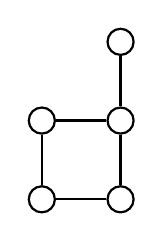
\begin{tikzpicture}[-,auto,node distance=1cm,
                    thick,main node/.style={circle,draw,font=\sffamily\small}]

  \node[main node] (1) {};
  \node[main node] (2) [right of=1] {};
  \node[main node] (3) [below of=1] {};
  \node[main node] (4) [right of=3] {};
  \node[main node] (5) [above of=2] {};
  \path[every node/.style={font=\sffamily\small}]
    (1) edge (2)
    	edge (3)
    (4) edge (2)
    	edge (3)
    (2) edge (5);
\end{tikzpicture}
\end{center}
\subsection{The Big Question with Planar Graphs}
Which graphs have a planar embedding?
\begin{ex}
$K_3$ is planar
\end{ex}
%K_3%
\begin{center}
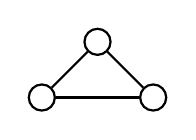
\begin{tikzpicture}[-,auto,node distance=1cm,
                    thick,main node/.style={circle,draw,font=\sffamily\small}]

  \node[main node] (1) {};
  \node[main node] (2) [below right of=1] {};
  \node[main node] (3) [below left of=1] {};
  \path[every node/.style={font=\sffamily\small}]
    (1) edge (2)
    	edge (3)
    (3) edge (2);
\end{tikzpicture}
\end{center}
\begin{ex}
$K_4$ is also planar (we can move edges and bend them)
\end{ex}
%K_4%
\begin{center}
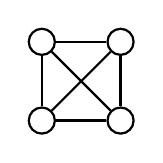
\begin{tikzpicture}[-,auto,node distance=1cm,
                    thick,main node/.style={circle,draw,font=\sffamily\small}]

  \node[main node] (1) {};
  \node[main node] (2) [right of=1] {};
  \node[main node] (3) [below of=1] {};
  \node[main node] (4) [below of=2] {};
  \path[every node/.style={font=\sffamily\small}]
    (1) edge (2)
    	edge (3)
    	edge (4)
    (2) edge (3)
    	edge (4)
    (3) edge (4);
\end{tikzpicture}
$\qquad=\qquad$
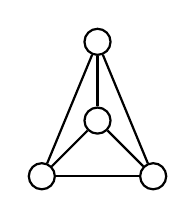
\begin{tikzpicture}[-,auto,node distance=1cm,
                    thick,main node/.style={circle,draw,font=\sffamily\small}]

  \node[main node] (1) {};
  \node[main node] (2) [above of=1] {};
  \node[main node] (3) [below right of=1] {};
  \node[main node] (4) [below left of=1] {};
  \path[every node/.style={font=\sffamily\small}]
    (1) edge (2)
    	edge (3)
    	edge (4)
    (2) edge (3)
    	edge (4)
    (3) edge (4);
\end{tikzpicture}
\end{center}
\noindent All cycles, paths, and trees are planar. But what about this graph:
\begin{center}
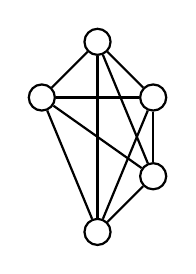
\begin{tikzpicture}[-,auto,node distance=1cm,
                    thick,main node/.style={circle,draw,font=\sffamily\small}]

  \node[main node] (1) {};
  \node[main node] (2) [above right of=1] {};
  \node[main node] (3) [below right of=2] {};
  \node[main node] (4) [below of=3] {};
  \node[main node] (5) [below left of=4] {};
  \path[every node/.style={font=\sffamily\small}]
    (1) edge (2)
    	edge (3)
    	edge (4)
    	edge (5)
    (2) edge (3)
    	edge (4)
    	edge (5)
    (3) edge (4)
    	edge (5)
    (4) edge (5);
\end{tikzpicture}
\end{center}
This graph, $K_5$, is \textit{not} planar. No matter how you draw it, there will always be a crossing. And actually, once you know $K_5$ is not planar, then $K_n$ is not planar for all $n \geq 5$. But why?
\subsubsection{Proposition 1}
\begin{center}
\textit{If G is planar and H is a subgraph of G, then H is planar}
\end{center}
\textbf{Proof:} finding any subgraph of $G$ will involve deleting edges and vertices from the planar embedding of $G$. Since no edges were crossed during this process, every subgraph must also be planar.
\subsubsection{Corollary 1}
\begin{center}
\textit{If G contains a non-planar subgraph H, then G is also non-planar}
\end{center}
\textbf{Proof:} this is the contrapositive of proposition 1.
\subsection{Finishing off the Lecture}
Corollary 1 proves the previous statement where $K_n$ is non-planar for all $n \geq 5$.\\
What about complete bipartite graphs ($K_{m,n}(m  \geq n)$)?
If $m$ or $n$ are less than 2, then it's planar.\\
What about $K_{3, 3}$? It's \textit{not} planar.
\begin{center}
\textit{$K_{3,3}$ and $K_5$ are the only ``reasons" a graph is not planar. In other words, if you can find $K_{3,3}$ or $K_5$ as a subgraph in a graph $G$, then $G$ is non-planar.}
\end{center}
%END%
\end{document}